\RequirePackage{luatex85}
\documentclass[tikz]{standalone}

\usepackage{siunitx}
\usetikzlibrary{arrows,calc,fit,positioning,backgrounds}

\usepackage{fontspec}
\setmainfont{Source Sans Pro}

\tikzset{
  >=latex,
  every path/.style={
    shorten <=2pt,shorten >=2pt,>=stealth
  },
  background rectangle/.style={fill=white},
  note/.style={
    font=\scriptsize
  },
  component/.style={
    rectangle,rounded corners,draw=black,
    text depth=0pt,
    minimum width=4cm,
    minimum height=8mm
  },
  small component/.style={
    component,
    text depth=0pt,
    font=\footnotesize,
    minimum width=20mm,
    minimum height=6mm,
  },
  dag/.style={
    component,draw=gray,line width=2pt,
    inner sep=3mm,
  },
  daglabel/.style={
    fill=white,
    text depth=0pt,
    font=\footnotesize,
    minimum height=6mm
  },
  prejob/.style={
    draw,
    minimum width=16mm,
    minimum height=6mm,
    text depth=0pt,
    font=\footnotesize,
    % append after command={
    %   \pgfextra
    %   \draw[shorten <=0pt, shorten >=0pt,black,rounded corners]%
    %   (\tikzlastnode.south east)%
    %     -- (\tikzlastnode.south)%
    %     -| (\tikzlastnode.west)%
    %     |- (\tikzlastnode.north)%
    %     -- (\tikzlastnode.north east);
    %   \endpgfextra
    % }
  },
  postjob/.style={
    draw,
    minimum width=16mm,
    minimum height=6mm,
    text depth=0pt,
    font=\footnotesize,
    % append after command={
    %   \pgfextra
    %   \draw[shorten <=0pt, shorten >=0pt,black,rounded corners]%
    %   (\tikzlastnode.north west)%
    %     -- (\tikzlastnode.north)%
    %     -| (\tikzlastnode.east)%
    %     |- (\tikzlastnode.south)%
    %     -- (\tikzlastnode.south west);
    %   \endpgfextra
    % }
  },
  mainjob/.style={
    component,
    rounded corners=0,
    minimum height=6mm,
    minimum width=25mm,
    text depth=0pt,
    font=\footnotesize,
  },
  optional/.style={
    dashed
  }
}


\begin{document}

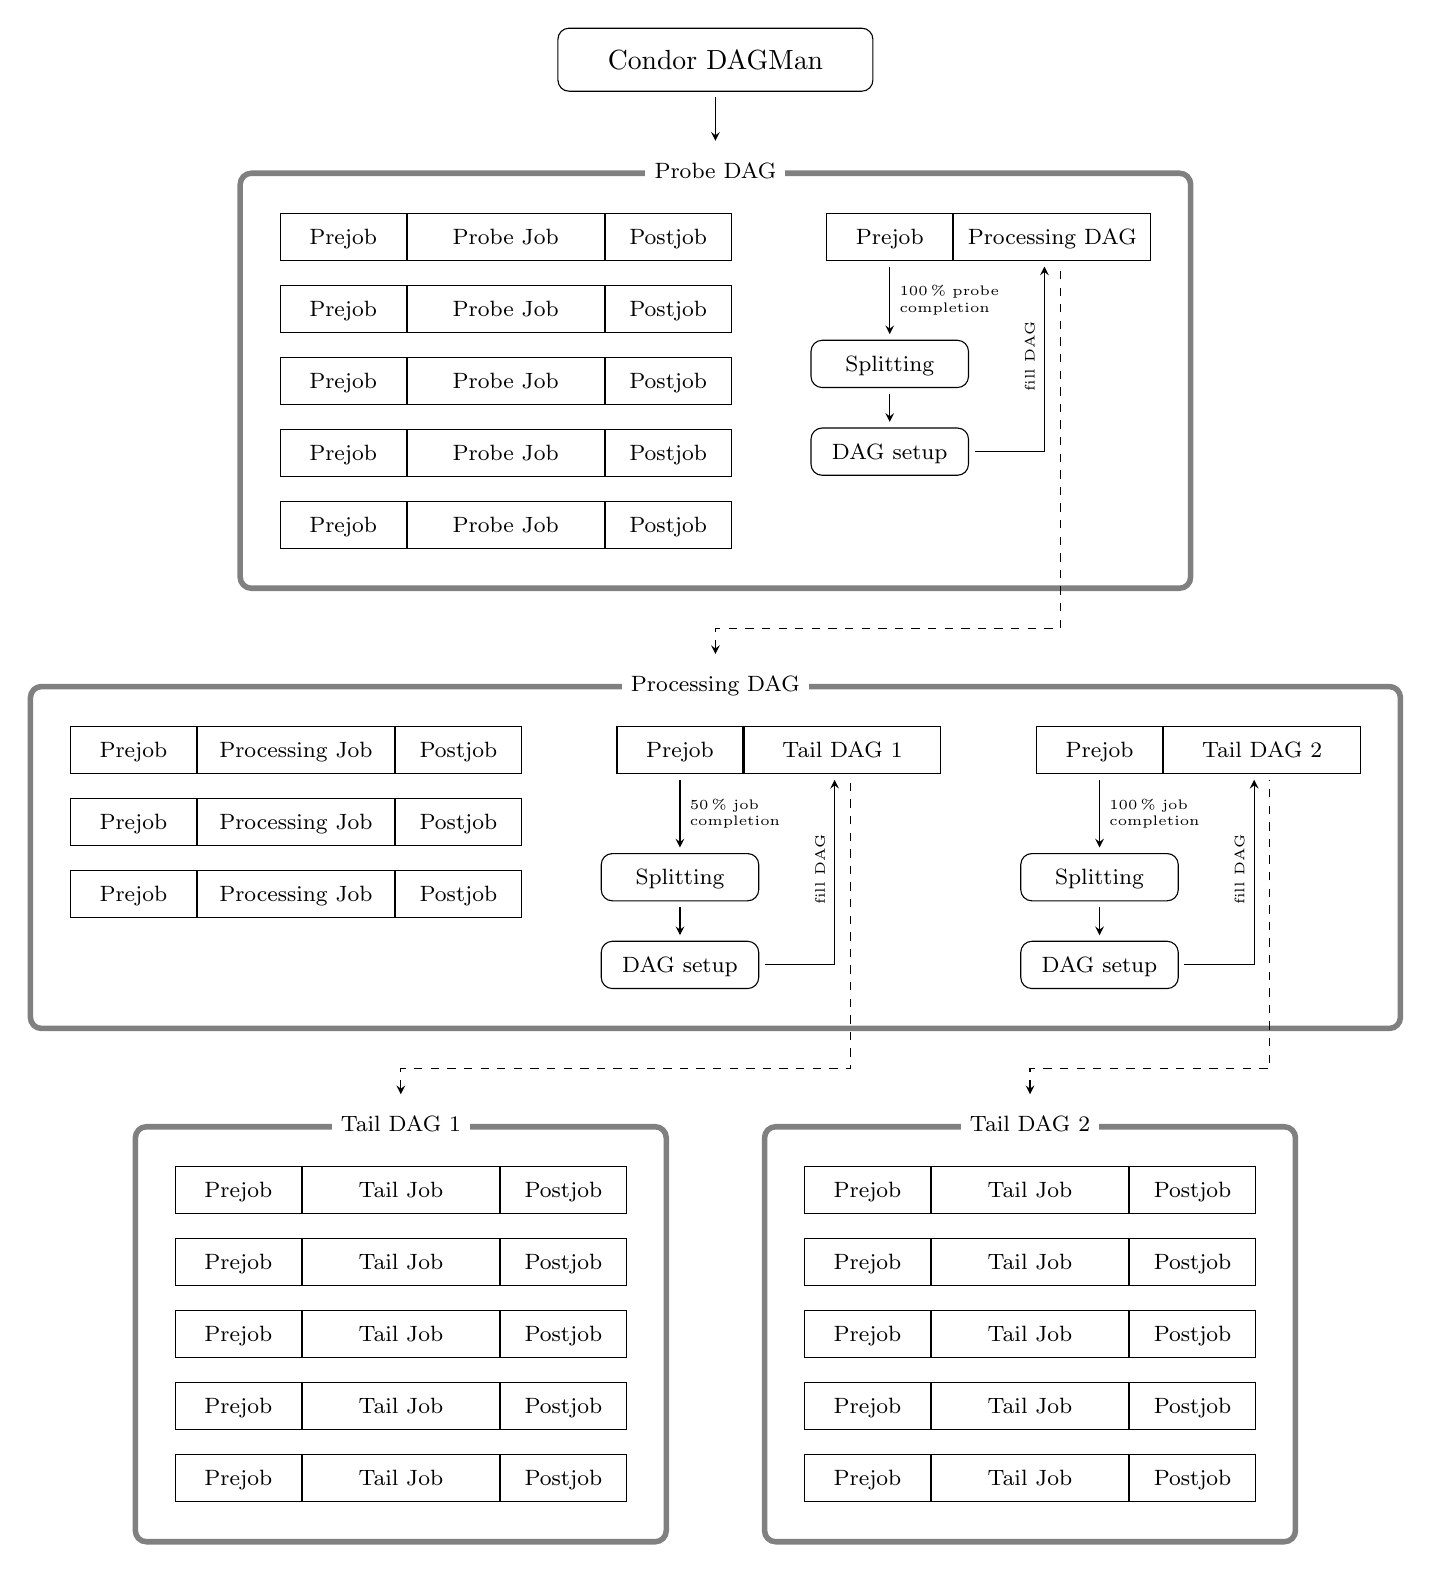
\begin{tikzpicture}
  \node[matrix,row sep=3mm] (t1) {
    \node[mainjob] (tail1-1-job) {Tail Job};
    \node[prejob,anchor=east] (tail1-1-pre) at (tail1-1-job.west) {Prejob};
    \node[postjob,anchor=west] (tail1-1-post) at (tail1-1-job.east) {Postjob};
    \\
    \node[mainjob] (tail1-2-job) {Tail Job};
    \node[prejob,anchor=east] (tail1-2-pre) at (tail1-2-job.west) {Prejob};
    \node[postjob,anchor=west] (tail1-2-post) at (tail1-2-job.east) {Postjob};
    \\
    \node[mainjob] (tail1-3-job) {Tail Job};
    \node[prejob,anchor=east] (tail1-3-pre) at (tail1-3-job.west) {Prejob};
    \node[postjob,anchor=west] (tail1-3-post) at (tail1-3-job.east) {Postjob};
    \\
    \node[mainjob] (tail1-4-job) {Tail Job};
    \node[prejob,anchor=east] (tail1-4-pre) at (tail1-4-job.west) {Prejob};
    \node[postjob,anchor=west] (tail1-4-post) at (tail1-4-job.east) {Postjob};
    \\
    \node[mainjob] (tail1-5-job) {Tail Job};
    \node[prejob,anchor=east] (tail1-5-pre) at (tail1-5-job.west) {Prejob};
    \node[postjob,anchor=west] (tail1-5-post) at (tail1-5-job.east) {Postjob};
    \\
  };

  \node[dag,inner sep=5mm,fit=(tail1-1-pre) (tail1-5-post)] (tail1dag) {};
  \node[daglabel] (tail1daglabel) at (tail1dag.north) {Tail DAG 1};

  \node[matrix,row sep=3mm,right=20mm of t1] (t2) {
    \node[mainjob] (tail2-1-job) {Tail Job};
    \node[prejob,anchor=east] (tail2-1-pre) at (tail2-1-job.west) {Prejob};
    \node[postjob,anchor=west] (tail2-1-post) at (tail2-1-job.east) {Postjob};
    \\
    \node[mainjob] (tail2-2-job) {Tail Job};
    \node[prejob,anchor=east] (tail2-2-pre) at (tail2-2-job.west) {Prejob};
    \node[postjob,anchor=west] (tail2-2-post) at (tail2-2-job.east) {Postjob};
    \\
    \node[mainjob] (tail2-3-job) {Tail Job};
    \node[prejob,anchor=east] (tail2-3-pre) at (tail2-3-job.west) {Prejob};
    \node[postjob,anchor=west] (tail2-3-post) at (tail2-3-job.east) {Postjob};
    \\
    \node[mainjob] (tail2-4-job) {Tail Job};
    \node[prejob,anchor=east] (tail2-4-pre) at (tail2-4-job.west) {Prejob};
    \node[postjob,anchor=west] (tail2-4-post) at (tail2-4-job.east) {Postjob};
    \\
    \node[mainjob] (tail2-5-job) {Tail Job};
    \node[prejob,anchor=east] (tail2-5-pre) at (tail2-5-job.west) {Prejob};
    \node[postjob,anchor=west] (tail2-5-post) at (tail2-5-job.east) {Postjob};
    \\
  };

  \node[dag,inner sep=5mm,fit=(tail2-1-pre) (tail2-5-post)] (tail2dag) {};
  \node[daglabel] (tail2daglabel) at (tail2dag.north) {Tail DAG 2};

  % probe dag done
  % processing dag start

  \coordinate (t12) at ($(t1.north)!0.5!(t2.north)$);

  \node[matrix,column sep=10mm,above=20mm of t12] (p) {
    \begin{scope}
      \node[mainjob] (job) {Processing Job};
      \node[prejob,anchor=east] (pre) at (job.west) {Prejob};
      \node[postjob,anchor=west] (post) at (job.east) {Postjob};

      \node[prejob,below=3mm of pre] (pre2) {Prejob};
      \node[mainjob,anchor=west] (job2) at (pre2.east) {Processing Job};
      \node[postjob,anchor=west] (post2) at (job2.east) {Postjob};

      \node[prejob,below=3mm of pre2] (pre3) {Prejob};
      \node[mainjob,anchor=west] (job3) at (pre3.east) {Processing Job};
      \node[postjob,anchor=west] (post3) at (job3.east) {Postjob};
    \end{scope}
    &

    \begin{scope}
      \node[prejob] (tdagfill1-pre) {Prejob};
      \node[mainjob,anchor=west] (tdagfill1) at (tdagfill1-pre.east) {Tail DAG 1};

      \node[small component,below=10mm of tdagfill1-pre] (t1split) {Splitting};
      \node[small component,below=5mm of t1split] (t1creat) {DAG setup};

      \draw[->] (tdagfill1-pre) -- (t1split) node [midway,right,font=\tiny,text width=20mm] {\SI{50}{\percent} job \\ completion};
      \draw[->] (t1split) -- (t1creat);
      \draw[->] (t1creat) -| ($(tdagfill1.south) - (1mm,0)$) node [near end,above,sloped,font=\tiny] {fill DAG};
    \end{scope}
    &

    \begin{scope}
      \node[prejob] (tdagfill2-pre) {Prejob};
      \node[mainjob,anchor=west] (tdagfill2) at (tdagfill2-pre.east) {Tail DAG 2};

      \node[small component,below=10mm of tdagfill2-pre] (t2split) {Splitting};
      \node[small component,below=5mm of t2split] (t2creat) {DAG setup};

      \draw[->] (tdagfill2-pre) -- (t2split) node [midway,right,font=\tiny,text width=20mm] {\SI{100}{\percent} job \\ completion};
      \draw[->] (t2split) -- (t2creat);
      \draw[->] (t2creat) -| ($(tdagfill2.south) - (1mm,0)$) node [near end,above,sloped,font=\tiny] {fill DAG};
    \end{scope}
    \\
  };

  % \draw[->] (tdagfill1) -- (tdagfill2-pre);

  \node[dag,inner sep=5mm,fit=(pre) (post3) (tdagfill2) (t2creat)] (maindag) {};
  \node[daglabel] (maindaglabel) at (maindag.north) {Processing DAG};

  % \draw[->] (probe5-post) -- (split);
  % \draw[->] (split) -- (creat);
  % \draw[->] (creat) -- (pre);
  % \draw[shorten <=0,->] ($(creat.east)!.5!(pre.west)$) |- (pre2);
  % \draw[shorten <=0,->] ($(creat.east)!.5!(pre.west)$) |- (pre3);

  \node[matrix,column sep=10mm,above=20mm of p] {
    \begin{scope}
      \node[mainjob] (probe1-job) {Probe Job};
      \node[prejob,anchor=east] (probe1-pre) at (probe1-job.west) {Prejob};
      \node[postjob,anchor=west] (probe1-post) at (probe1-job.east) {Postjob};

      \node[mainjob,below=3mm of probe1-job] (probe2-job) {Probe Job};
      \node[prejob,anchor=east] (probe2-pre) at (probe2-job.west) {Prejob};
      \node[postjob,anchor=west] (probe2-post) at (probe2-job.east) {Postjob};

      \node[mainjob,below=3mm of probe2-job] (probe3-job) {Probe Job};
      \node[prejob,anchor=east] (probe3-pre) at (probe3-job.west) {Prejob};
      \node[postjob,anchor=west] (probe3-post) at (probe3-job.east) {Postjob};

      \node[mainjob,below=3mm of probe3-job] (probe4-job) {Probe Job};
      \node[prejob,anchor=east] (probe4-pre) at (probe4-job.west) {Prejob};
      \node[postjob,anchor=west] (probe4-post) at (probe4-job.east) {Postjob};

      \node[mainjob,below=3mm of probe4-job] (probe5-job) {Probe Job};
      \node[prejob,anchor=east] (probe5-pre) at (probe5-job.west) {Prejob};
      \node[postjob,anchor=west] (probe5-post) at (probe5-job.east) {Postjob};
    \end{scope}
    &

    \begin{scope}
      \node[prejob] (pdagfill-pre) {Prejob};
      \node[mainjob,anchor=west] (pdagfill) at (pdagfill-pre.east) {Processing DAG};

      \node[small component,below=10mm of pdagfill-pre] (psplit) {Splitting};
      \node[small component,below=5mm of psplit] (pcreat) {DAG setup};
    \end{scope}
    \\
  };

  \node[dag,inner sep=5mm,fit=(probe1-pre) (probe5-post) (pcreat) (pdagfill)] (probedag) {};
  \node[daglabel] (probedaglabel) at (probedag.north) {Probe DAG};

  \draw[->] (pdagfill-pre) -- (psplit) node [midway,right,font=\tiny,text width=20mm] {\SI{100}{\percent} probe \\ completion};
  \draw[->] (psplit) -- (pcreat);
  \draw[->] (pcreat) -| ($(pdagfill.south) - (1mm,0)$) node [near end,above,sloped,font=\tiny] {fill DAG};

  \node[component,above=of probedag] (dagm) {Condor DAGMan};

  \draw[->] (dagm) -- (probedaglabel);

  \draw[<-,dashed] (tail1daglabel) -- ++(0,7mm) -| ($(tdagfill1.south) + (1mm,0)$);
  \draw[<-,dashed] (tail2daglabel) -- ++(0,7mm) -| ($(tdagfill2.south) + (1mm,0)$);
  \draw[<-,dashed] (maindaglabel) -- ++(0,7mm) -| ($(pdagfill.south) + (1mm,0)$);
\end{tikzpicture}

\end{document}
